
%%%%%%%% ICML 2015 EXAMPLE LATEX SUBMISSION FILE %%%%%%%%%%%%%%%%%
%%%%%%%%%%%%%%%%%%%%%%%%%%%%%%%%%%%%%%%%%%%%%%%%%%%%%%%%%%%%%%%%%%

\documentclass{article}

\usepackage{times}
\usepackage{graphicx}
\usepackage{subfigure} 

% For citations
\usepackage{natbib}
\usepackage[utf8]{inputenc}

% For algorithms
%\usepackage{algorithm}
%\usepackage{algorithmic}
% Packages hyperref and algorithmic misbehave sometimes.  We can fix
% this with the following command.
%\newcommand{\theHalgorithm}{\arabic{algorithm}}

\usepackage{hyperref}
\usepackage{amsmath}
\usepackage{amssymb}

\def \N {\mathbb{N}}
\def \Nbr {\mathcal{N}}
\def \Q {\mathbb{Q}}
\def \F {\mathbb{F}}
\def \then {\implies &}
\def \oif {\Longleftrightarrow &\,}
\def \given {\text{Given }&}
\def \assume {\text{Assume }&}
\def \thfr {\therefore &\enskip}
\def \bij {\leftrightarrow}
\def \inj {\rightarrowtail}
\def \sur {\twoheadedrightarrow}
\def \Z {\mathbb{Z}}
\def \R {\mathbb{R}}
\def \C {\mathbb{C}}
\def \D {\mathbb{D}}
\def \iff {\Longleftrightarrow}
\def \kron {\boldsymbol\delta}
\def \id {\text{id}}

\def\Tx{\textbf{x}}
\def\Ty{\textbf{y}}
\def\quotient{\mathclose{}/\mathopen{}}
\def\Tf{\textbf{f}}
\def\Th{\textbf{h}}
\def\Tg{\textbf{g}}
\def\sumn{\sum_{n=0}^\infty}
\def\limn{\lim_{n\rightarrow\infty}}
\def\prodn{\prod_{n=0}^\infty}
\DeclareMathOperator\adj{adj}

\newcommand{\stc}[1]{\widetilde{#1}}   
\newcommand{\pa}[1]{ \left({#1}\right) }
\newcommand{\set}[2]{ \left\{ #1 \,\middle|\, #2 \right\} }
\newcommand{\shift}[1]{&\quad & \text{#1}\\}
\newcommand{\lem}[1]{\text{\textbf{L.\ref{#1}}}}
\newcommand{\card}[1]{\left\vert{#1}\right\vert}
\newcommand{\Ps}[1]{\mathcal{P}\left({ #1 }\right)}
\newcommand{\colv}[1]{\begin{pmatrix} #1 \end{pmatrix}}
\newcommand{\mat}[1]{\begin{pmatrix} #1 \end{pmatrix}}
\newcommand{\detmat}[1]{\begin{vmatrix} #1 \end{vmatrix}}
\newcommand{\spanb}[1]{\text{span}\{ #1 \}}
\newcommand{\abs}[1]{\left|#1\right|}
\newcommand{\Inner}[1]{\langle #1 \rangle}
\newcommand{\Innercpy}[1]{\langle #1, #1 \rangle}
\newcommand{\conj}[1]{{\overline{#1}}}

\DeclareMathOperator{\Tr}{tr}
\DeclareMathOperator{\Dim}{dim}
\DeclareMathOperator{\Rank}{rank}
\DeclareMathOperator{\Ker}{ker}
\DeclareMathOperator{\Diam}{diam}
\DeclareMathOperator{\Diag}{diag}
\DeclareMathOperator{\Int}{int}
\DeclareMathOperator{\Clo}{clo}
\DeclareMathOperator{\sgn}{sgn}
\DeclareMathOperator{\MyRe}{Re}
\DeclareMathOperator{\MyIm}{Im}
\DeclareMathOperator{\res}{res}

% Employ the following version of the ``usepackage'' statement for
% submitting the draft version of the paper for review.  This will set
% the note in the first column to ``Under review.  Do not distribute.''
%\usepackage{icml2015} 

% Employ this version of the ``usepackage'' statement after the paper has
% been accepted, when creating the final version.  This will set the
% note in the first column to ``Proceedings of the...''
\usepackage[accepted]{icml2015}


% The \icmltitle you define below is probably too long as a header.
% Therefore, a short form for the running title is supplied here:
\icmltitlerunning{Commodities Forecasting with GDELT}

\begin{document} 

\twocolumn[
\icmltitle{Commodities Forecasting from Non-Financial World News from GDELT}

% It is OKAY to include author information, even for blind
% submissions: the style file will automatically remove it for you
% unless you've provided the [accepted] option to the icml2015
% package.
\icmlauthor{Vladimir Feinberg}{vyf@princeton.edu}
\icmladdress{Princeton University}
\icmlauthor{Daway Chou-Ren}{dchouren@princeton.edu}
\icmladdress{Princeton University}

% You may provide any keywords that you 
% find helpful for describing your paper; these are used to populate 
% the "keywords" metadata in the PDF but will not be shown in the document
\icmlkeywords{GDELT, commodities, finance, forecasting, clustering, machine learning, ICML}

\vskip 0.3in
]

\begin{abstract} 

%TODO fill in abstract.

\end{abstract} 

%TODO review below
% Submissions must be in PDF.
% The maximum paper length is \textbf{8 pages excluding references, and 10 pages including references} (pages 9 and 10 must contain only references).
% Do \textbf{not include author information or acknowledgments} in your initial submission. 
% Your paper should be in \textbf{10 point Times font}.
% Make sure your PDF file only uses Type-1 fonts.
% Place figure captions {\em under} the figure (and omit titles from inside the graphic file itself).  Place table captions {\em over} the table.
% References must include page numbers whenever possible and be as complete as possible.  Place multiple citations in chronological order.  
% Do not alter the style template; in particular, do not compress the paper format by reducing the vertical spaces.

\section{Introduction}
 
% Daway 
Financial data prediction is appealing both for its challenging nature and for its practical applications. Because market dynamics are complex and random, accurate price prediction is difficult. There are two types of market prediction techniques: fundamental analysis, which relies on an asset's data for forecasting, and technical analysis, which relies on historical trends to exploit market timing \cite{schumaker2009textual}. This paper examines the use of news data to augment technical analysis for prediction of commodity prices. We assume there is a set of news basis vectors that is stable over time which can be used for this purpose. %TODO: keep last sentence?

We focus on a comprehensive set of non-economic news data unrelated to financial markets, interest rates, stock prices, and the like. In particular, we will analyze whether a summary of a day's news topics is predictive of commodity prices the next day. To avoid losing information about the significance of singular events, we will rely on the sentiment analysis already applied to our dataset to calculate how each news event should be weighted in a daily news summary.

\subsection{Commodity Prediction}
We choose to predict commodities prices because while various studies have analyzed the effect of news on stock prices \cite{mcqueen1993stock} and foreign exchange rates \cite{kamruzzaman2003svm}, relatively little work has looked at applying news data to the prediction of the similar commodities market. The use non-economic news because the influence of economic news has already been examined in the past by many researchers \cite{gidofalvi2001using}\cite{schumaker2009textual}\cite{bollen2011twitter}\cite{hagenau2012automated}. We believe real-time news information has predictive power for commodity prices, because, since commodities, by definition, must be extracted or produced by countries, it is likely that underlying factors of their production rates will be captured by local news, especially reporting on crisis events. Prices are also sensitive to current conditions because the supply and demands that drive them are inelastic, or unaffected by changes in price \cite{chen2008can}. 

\subsection{GDELT Dataset}
We draw news from the Global Database of Events, Language, and Tone \cite{GDELT}, which aggregates news from broadcast, print, and web sources across 100 languages and parses out features to describe each news event. Each news event has 58 features which can be broadly divided into either topical or importance-related data. Topical data might include the two actors involved in an event, the general sentiment of the language used, the location of actors, or broad categorization of the type of event occurring (trade agreement, violent action, etc) in categorical codes (CAMEO codes). Importance-related features deal with the magnitude of the event and are drawn from metrics such as the number of news sources mentioning the event, or the total number of articles written about it. GDELT is available for free and uses a variety of international news sources with daily updates, and contains more than 250 million events from 1979 to present, or roughly 100,000 per day. GDELT's predictive potential for financial markets has been positively assessed by researchers who used GDELT to examine the impacts of the June 2013 Southeast Asian heat wave and the December 2013 Indian riots and the effect they had on the Singapore stock market \cite{phua2014visual}.

 
\section{Motivating Analysis}

% Vlad

\subsection{GDELT Dataset}

\subsubsection{Sparsity in GDELT}

The space of news events spanned by all columns in GDELT is much larger than the subspace we expect news to lie on. Confirming these suspicions is important because it would indicate a need to reduce the dimensionality of the data set we are working with.

Classical dimensionality reduction was not tractable to apply to a dataset of this size - the highly categorical nature of the dataset results in a large dimensional expansion when preparing numeric inputs to the algorithms. A fast neighborhood-embedding method, tSNE, relies only on a metric between data points. Unfortunately, its runtime and space consumption grows exponentially in the reduced dimension, and extremely small dimensions yielded poor results \yrcite{van2008visualizing}.

However, it is critical to observe some sparsity in the GDELT space to confirm our clustering-based approach.

We guessed that there are likely to be at least two modes of low-dimensional interactions in the data: (1) that actors only interact within small cliques and (2) that each actors to small sets of events. We conducted this initial analysis on a random sample of days before August 2015 to avoid making conclusions that overfit the test data.

\begin{figure}[ht]
\vskip 0.2in
\begin{center}
%\centerline{\includegraphics[width=\columnwidth]{}}
\caption{
BOX WHISKER HERE. DESCRIBE 5 FIGURE SUMMARIES, OUTLIER
}
\end{center}
\vskip -0.2in
\label{fig:events-per-actor}
\end{figure} 


\begin{figure}[ht]
\vskip 0.2in
\begin{center}
%\centerline{\includegraphics[width=\columnwidth]{}}
\caption{TODO: take another random sample, histogram it. Describe summary stats. number of Distinct events per actor.}
\end{center}
\vskip -0.2in
\label{fig:events-per-actor}
\end{figure} 


As Figure \ref{fig:actors-per-actor} demonstrates, actor count is heavily skewed distribution. This gives us confidence in (1) for the sampled days. We conduct a similar inspection for the number of unique CAMEO coded events per actor in Figure \ref{fig:events-per-actor}:

\begin{figure}[ht]
\vskip 0.2in
\begin{center}
%\centerline{\includegraphics[width=\columnwidth]{}}
\caption{TODO: take another random sample, histogram it. Describe summary stats. number of Distinct events per actor.}
\end{center}
\vskip -0.2in
\label{fig:events-per-actor}
\end{figure} 

In addition to more compact data representation and reduction of noise, dimensionality reduction has several other attractive features for this dataset. First, it enables us to work in a continuous space of reduced-dimension tuples of real values, which is much easier for model generation than partially categorical variables. Secondly, the large volume of the data set implies that any size reductions that can be gained will result in more manageable data pipelines

\subsection{Bloomberg Commodity Prices}

up and down spikes

normally distributed about 0

\section{Related Work}

% Daway
On the whole, predicting any financial market has proven to be difficult. Simon's work encapsulates many of the inherent problems. Model evaluation cannot rely on using normal RMSE metrics, which might suffer from lag problems, but must either demonstate ability to generate profit through a trading scheme or demonstrate an ability to correctly predict directionality for desired trading period times. Simon identifies a training period of 3 years and a test period of 6 months as optimal \cite{forex_neuralnets}.

\noindent In an examination of the potential for technical approaches to predict pricing movements, Gidofalvi found that a 20 minute period before and after the release of financial news allowed for a weak prediction of price movements \cite{gidofalvi2001using}. It was found by McQueen and Roley that fundamental macroeconomic news has little impact on stock prices but that other news types have effects dependent on responses of expected flows relative to equity discount rates \cite{mcqueen1993stock}.\\

\noindent In addition to Phua et al's work in identifying crisis points in Singapore's stock market, Schumaker and Chen were able to demonstrate 57\% directional accuracy when using news articles to predict S\&P500 stocks in Gidofalvi's 20 minute period \cite{schumaker2009textual}. Bollen et al also achieved an accuracy of 86.7\% when incorporating semantic mood data from Twitter \cite{bollen2011twitter}. Other research has focused on extracting semantics from blogs or financial news. Hagenau et al show that context-specific feature extraction from news can reduce overfitting of models \cite{hagenau2012automated}.\\

\noindent The work done by Phua et al is important for validating GDELT in particular as a valid news source for market prediction. Topic analysis shows that GDELT includes impactful events across multiple iterations of clustering (thus correctly assigning impactful events large magnitudes) and also correctly chronologically tracks changing magnitudes. Term extraction from news sources is shown to be relevant using concept link exploration. Phua et all do find that not all significant events can be discovered by GDELT. They were also unable to verify that quality for semantic score assignments was high.

\section{Methods}

% Vlad (+ Daway for pictures)


analysis done on prefix of days to prevent overfitting \cite{leetaru2013gdelt}

(summary info, description of columns)

(description of columns we actually used)

\begin{figure}[ht]
\vskip 0.2in
\begin{center}
\centerline{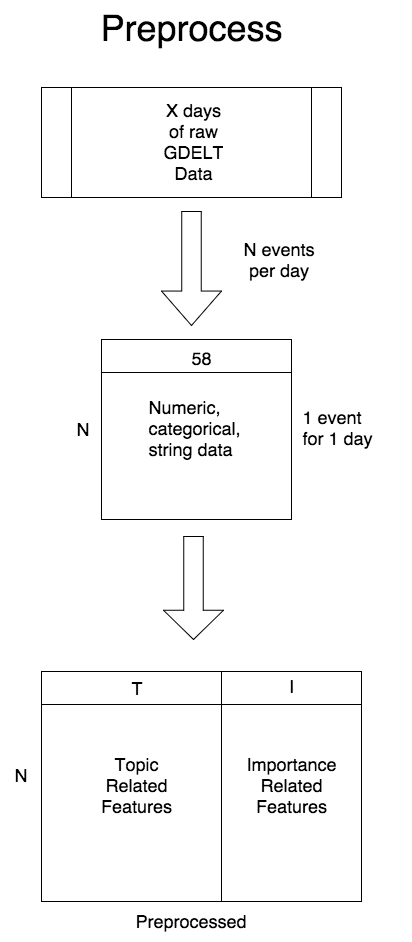
\includegraphics[scale=0.15]{images/preprocess_vertical.png}}
\caption{Preprocess stage}
\end{center}
\vskip -0.2in
\label{fig:preprocess}
\end{figure} 


\begin{figure}[ht]
\vskip 0.2in
\begin{center}
\centerline{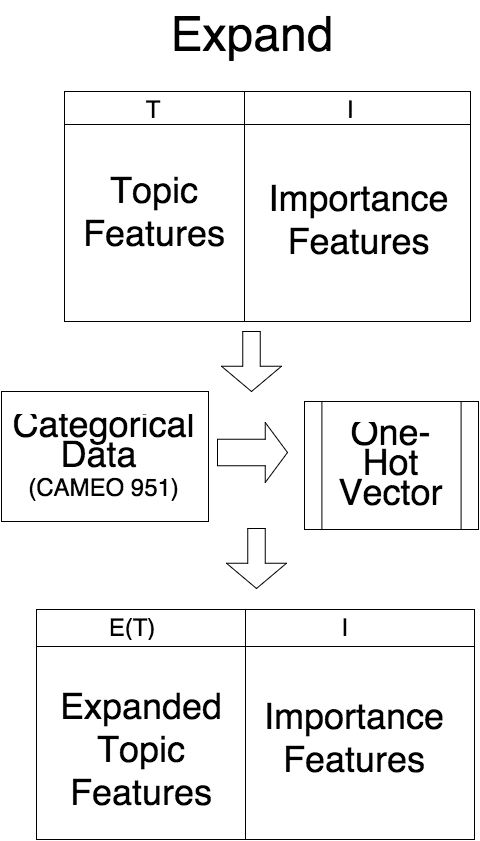
\includegraphics[width=\columnwidth]{images/expand_vertical.png}}
\caption{Expand stage}
\end{center}
\vskip -0.2in
\label{fig:exapand}
\end{figure} 




\begin{figure}[ht]
\vskip 0.2in
\begin{center}
\centerline{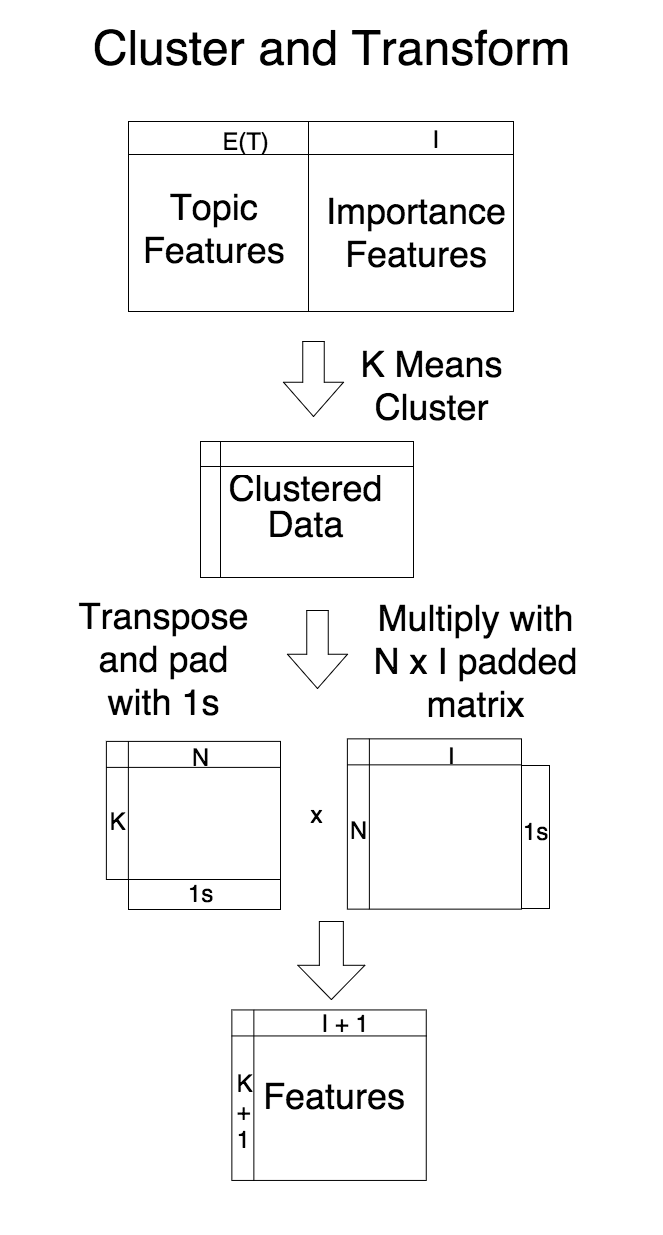
\includegraphics[scale=0.15]{images/cluster_and_transform_vertical.png}}
\caption{Summarization stage}
\end{center}
\vskip -0.2in
\label{fig:summarization}
\end{figure} 

\section{Evaluation}


analysis done on prefix of days to prevent overfitting 

\section{Results}

% Daway
% remember to add the disclaimer on the current results

%TODO remember to add runtime info later (not for first run)

\section{Future Work}

% Vlad
\subsection{Improving the Prediction Models}
We have tried different window sizes for both training and testing as well as moving the windows instead of fixing them. We also tried using PCA for LM and ARIMA but found that using Lasso once the orders of AR and MA are determined to be more efficient. Our binary accuracy results are on-par with the state-of-the-art ones. However, it is clear that our prediction, for the simple log return data, is most from the time series lags itself and not GDELT. The sparser our usage of GDELT is, the higher our testing results are. Therefore, we have to either analyze different time series (discussed later in this section) or try to estimate different features of the time series such as extreme values or peaks in the log return. For example, we could work on a logistic regression that classifies days in the top $10\%$ in terms of log return value, as "high", days in the bottom $10\%$ as low and the rest as "medium". In this case, we would be doing two classifiers, one on the "high" and one on the "low" in a similar fashion to exemplar SVM, where we train the high/low with so many negative examples that it has a higher certainty where predicting a peak. Our final result would indicate whether there are peaks (high or low) or if the trading activity is rather normal (medium) or if our results conflict (we get positive for both high and low). Only in the first case where we are sure about one kind of the peaks would we consider the prediction for our trading strategy.

\subsection{Infinite Gaussian Mixture Model}
For clustering news events we have relatively little information for deciding how many clusters there should be. In our $K$-means model, we do a parameter search for values of $K$ from 10 to 5000 on a logarithmic scale. Ideally we would be able to use an infinite Gaussian mixture model that takes in a hyperparameter for a clustering coefficient and automatically determines the number of clusters and therefore remove the need for this imprecise parameter search. 

We attempted using a Dirichlet Process GMM but the implementation we attempted to use was intractable given our computing power. We may attempt to optimize the parameters of the DPGMM in the future or work on limiting the model's training set further. 

\subsection{Filtering GDELT by Commodity}
Up to now, we have been sampling the entire GDELT dataset for news events in order to predict the movement in commodity prices (e.g. silver). Since GDELT contains a large variety of news topics, the majority of the news articles within each day are not related to the specific commodity that we study. A more accurate way to predict the commodity prices would be to implement a filtering pipeline that removes irrelevant news items. This can be achived with natural language processing by selecting news articles that have keywords such as ``silver" and ``commodity". This approach should improve our prediction accuracy because it would remove a significant portion of the noise in GDELT.




\subsection{Software and Data}

All code used is available at \hyperref[https://github.com/vlad17/COS513-Finance]{https://github.com/vlad17/COS513-Finance}. GDELT provides free access to its database as well: \hyperref[http://data.gdeltproject.org/events/index.html]{http://data.gdeltproject.org/events/index.html}.

Commodities pricing data is retrieved using the \texttt{R} package quantmod, which pulls historical prices using Yahoo: \hyperref[http://www.quantmod.com/]{http://www.quantmod.com/}

%TODO add a bunch more references everywhere to defend all our claims.

% Acknowledgements should only appear in the accepted version. 
% \section*{Acknowledgments} 

% In the unusual situation where you want a paper to appear in the
% references without citing it in the main text, use \nocite
% \nocite{langley00}

\bibliography{biblio}
\bibliographystyle{icml2015}

\end{document} 

% EXAMPLE FOOTNOTE
%\footnote{Example footnote should have full sentences.}

% EXAMPLE IMAGES
%\begin{figure}[ht]
%\vskip 0.2in
%\begin{center}
%\centerline{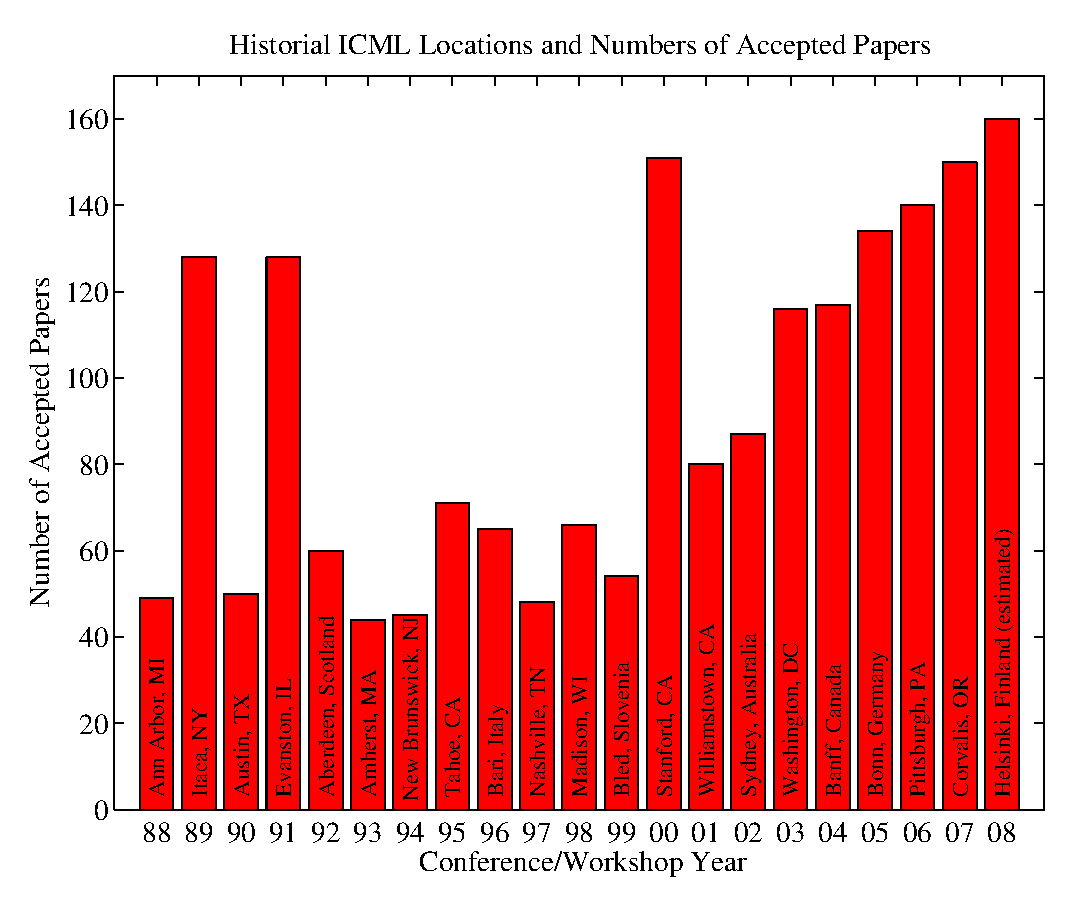
\includegraphics[width=\columnwidth]{icml_numpapers}}
%\caption{Historical locations and number of accepted papers for International
%  Machine Learning Conferences (ICML 1993 -- ICML 2008) and
%  International Workshops on Machine Learning (ML 1988 -- ML
%  1992). At the time this figure was produced, the number of
%  accepted papers for ICML 2008 was unknown and instead estimated.}
%\label{icml-historical}
%\end{center}
%\vskip -0.2in
%\end{figure} 

%Citations within the text should include the authors' last names and
%year. If the authors' names are included in the sentence, place only
%the year in parentheses, for example when referencing Arthur Samuel's
%pioneering work \yrcite{Samuel59}. Otherwise place the entire
%reference in parentheses with the authors and year separated by a
%comma \cite{Samuel59}. List multiple references separated by
%semicolons \cite{kearns89,Samuel59,mitchell80}. Use the `et~al.'
%construct only for citations with three or more authors or after
%listing all authors to a publication in an earlier reference \cite{MachineLearningI}.

% EXAMPLE TABLE
%\begin{table}[t]
%\caption{Classification accuracies for naive Bayes and flexible 
%Bayes on various data sets.}
%\label{sample-table}
%\vskip 5in
%\begin{center}
%\begin{small}
%\begin{sc}
%\begin{tabular}{lcccr}
%\hline
%\abovespace\belowspace
%Data set & Naive & Flexible & Better? \\
%\hline
%\abovespace
%Breast    & 95.9$\pm$ 0.2& 96.7$\pm$ 0.2& $\surd$ \\
%Cleveland & 83.3$\pm$ 0.6& 80.0$\pm$ 0.6& $\times$\\
%Glass2    & 61.9$\pm$ 1.4& 83.8$\pm$ 0.7& $\surd$ \\
%Credit    & 74.8$\pm$ 0.5& 78.3$\pm$ 0.6&         \\
%Horse     & 73.3$\pm$ 0.9& 69.7$\pm$ 1.0& $\times$\\
%Meta      & 67.1$\pm$ 0.6& 76.5$\pm$ 0.5& $\surd$ \\
%Pima      & 75.1$\pm$ 0.6& 73.9$\pm$ 0.5&         \\
%\belowspace
%Vehicle   & 44.9$\pm$ 0.6& 61.5$\pm$ 0.4& $\surd$ \\
%\hline
%\end{tabular}
%\end{sc}
%\end{small}
%\end{center}
%\vskip -0.1in
%\end{table}